\documentclass[a4paper,12pt]{extarticle}
\usepackage[utf8x]{inputenc}
\usepackage[T1,T2A]{fontenc}
\usepackage[russian]{babel}
\usepackage{hyperref}
\usepackage{indentfirst}
\usepackage{listings}
\usepackage{color}
\usepackage{xcolor}
\usepackage{here}
\usepackage{array}
\usepackage{multirow}
\usepackage{graphicx}
\usepackage{amsmath}

\hypersetup{
    colorlinks = false,
    linkbordercolor = {white}
}

\definecolor{string}{HTML}{B40000} % цвет строк в коде
\definecolor{comment}{HTML}{008000} % цвет комментариев в коде
\definecolor{keyword}{HTML}{1A00FF} % цвет ключевых слов в коде
\definecolor{morecomment}{HTML}{8000FF} % цвет include и других элементов в коде
\definecolor{сaptiontext}{HTML}{FFFFFF} % цвет текста заголовка в коде
\definecolor{сaptionbk}{HTML}{999999} % цвет фона заголовка в коде
\definecolor{bk}{HTML}{FFFFFF} % цвет фона в коде
\definecolor{frame}{HTML}{999999} % цвет рамки в коде
\definecolor{brackets}{HTML}{B40000} % цвет скобок в коде

\usepackage{caption}
\renewcommand{\lstlistingname}{Программа} % заголовок листингов кода

\bibliographystyle{ugost2008ls}

\usepackage{listings}
\lstset{ %
	extendedchars=\true,
	keepspaces=true,
	language=Python,						% choose the language of the code
	% Цвета
	keywordstyle=\color{keyword}\ttfamily\bfseries,
	%stringstyle=\color{string}\ttfamily,
	stringstyle=\ttfamily\color{red!50!brown},
	commentstyle=\color{comment}\ttfamily\itshape,
	morecomment=[l][\color{morecomment}]{\#},
	basicstyle=\footnotesize,		% the size of the fonts that are used for the code
	numbers=left,					% where to put the line-numbers
	numberstyle=\footnotesize,		% the size of the fonts that are used for the line-numbers
	stepnumber=1,					% the step between two line-numbers. If it is 1 each line will be numbered
	numbersep=5pt,					% how far the line-numbers are from the code
	backgroundcolor=\color{white},	% choose the background color. You must add \usepackage{color}
	showspaces=false				% show spaces adding particular underscores
	keywordstyle=color{blue}\bfseries, 
	showstringspaces=false,			% underline spaces within strings
	showtabs=false,					% show tabs within strings adding particular underscores
	frame=single,          		% adds a frame around the code
	tabsize=2,						% sets default tabsize to 2 spaces
	captionpos=t,					% sets the caption-position to top
	breaklines=true,				% sets automatic line breaking
	breakatwhitespace=false,		% sets if automatic breaks should only happen at whitespace
	escapeinside={\%*}{*)},			% if you want to add a comment within your code
	postbreak=\raisebox{0ex}[0ex][0ex]{\ensuremath{\color{red}\hookrightarrow\space}},
	texcl=true,
	inputpath=listings,                     % директория с листингами
}

\usepackage[left=2cm,right=2cm,
top=2cm,bottom=2cm,bindingoffset=0cm]{geometry}

%% Нумерация картинок по секциям
\usepackage{chngcntr}
\counterwithin{figure}{section}
\counterwithin{table}{section}

%%Точки нумерации заголовков
\usepackage{titlesec}
\titlelabel{\thetitle.\quad}
\usepackage[dotinlabels]{titletoc}

%% Оформления подписи рисунка
\addto\captionsrussian{\renewcommand{\figurename}{Рисунок}}
\captionsetup[figure]{labelsep = period}

%% Подпись таблицы
\DeclareCaptionFormat{hfillstart}{\hfill#1#2#3\par}
\captionsetup[table]{format=hfillstart,labelsep=newline,justification=centering,skip=-10pt,textfont=bf}

%% Путь к каталогу с рисунками
\graphicspath{{fig/}}

\begin{document}	% начало документа

% Титульная страница
%\begin{titlepage}	% начало титульной страницы

	\begin{center}		% выравнивание по центру

		Санкт-Петербургский Национально Исследовательский Университет\\
		информационных технологий, механики и оптики \\
		Кафедра систем управления и информатики\\[3cm]
		% название института, затем отступ 6см
		
		\huge \textbf{РЕФЕРАТ}\\[0.5cm]
		\large Электромеханические системы\\[0.1cm]
		\large Система автоматического управления квадракоптера Parrot ARDrone 2.0\\[2cm]

	\end{center}


	\begin{flushright} % выравнивание по правому краю
%		\begin{minipage}{0.5\textwidth} % врезка в половину ширины текста
%			\begin{flushleft} % выровнять её содержимое по левому краю

				\large Выполнили студенты группы P3335\\
				\large А.М. Зенкин\\[0.5cm]
				\large К.В. Карпов\\[0.5cm]
				
				\large Принял  к.т.н., доцент кафедры СУиР\\
				\sign[4cm]\large  М.С. Чежин\\
				\large Оценка: \sign\\
				«\underline{\hspace{0.7cm}}» \underline{\hspace{2cm}} \the\year г.

%			\end{flushleft}
%		\end{minipage}
	\end{flushright}
	
	\vfill % заполнить всё доступное ниже пространство

	\begin{center}
	\large Санкт-Петербург\\
	\large \the\year % вывести дату
	\end{center} % закончить выравнивание по центру

\thispagestyle{empty} % не нумеровать страницу
%\end{titlepage} % конец титульной страницы
\newpage


% Содержание
% Содержание
\renewcommand\contentsname{\centerline{Содержание}}
\tableofcontents
\thispagestyle{fancy}
\newpage




\section{Цель работы}
Ознакомление с пакетом прикладных программ SIMULINK и основными приемами моделирования линейных динамических систем.


\section{Варианты параметров}

$n = 3$, $a_0 = 7$, $a_1 = 5$, $a_2 = 2$, $b_0 = 10$, $b_1 = 3$, $b_2 = 1.5$, $y(0) = 1$, $\dot{y}(0) = -0.5$, $\ddot{y}(0) = 0$\\

$n = 2$,  $A = \begin{bmatrix}
				0 & 1\\
				-5 & -0.5
				\end{bmatrix}$, $B = \begin{bmatrix}
									0.5\\
									1
									\end{bmatrix}$, $C^T = \begin{bmatrix}
															5\\
															0.5
															\end{bmatrix}$\\
															
$x_1(0) = 0.2$, $x_2(0) = -0.1$, $x_3(0) = -$


\section{Ход выполнения работы}

\subsection{Модель вход-выход}

\subsubsection{Математическая модель:}

\begin{equation}
	\begin{split}	
&\dddot{y} + 2\ddot{y} + 5\dot{y} + 7y = 1.5\ddot{u} + 3\dot{u} + 10u\\
&s^3y + 2s^2y + 5sy = 1.5s^2u + 3su + 10u | :s^3\\
&y = \frac{1}{s}(1.5u - 2y) + \frac{1}{s^2}(3u - 5y) + \frac{1}{s^3}(10u - 7y)\\
&z_1 = y\\
&z_1(0) = y(0) = 1\\
&\dot{y} = \dot{z_1} = \dot{z_2} + 1.5u - 2y\\
&z_2 = \dot{y} - 1.5u + 2y\\
&z_2(0) = \dot{y}(0) - 1.5u(0) + 2y(0) = -0.5 + 2*1 - 0 = 1.5\\
&z_2 = z_3 - 5y + 3u\\
&z_3 = /dot{z_2} + 5y -3u\\
&z_3 = \ddot{y} - 1.5\dot{u} + 2\dot{y} + 5\dot{y} -3\dot{u}\\
&z_3(0) = \ddot{y}(0) - 1.5\dot{u}(0) + 2\dot{y}(0) + 5\dot{y}(0) - 3\dot{u}(0) = 0 -0 - 1 - 5*0.5 - 0 = -3.5\\
	\end{split}
\end{equation}

\subsubsection{Моделирование системы при двух видах входного воздействия — u = 2sin(t)  и u = 1(t) — и нулевых начальных условиях:}

\begin{figure}[H]
	\begin{center}
		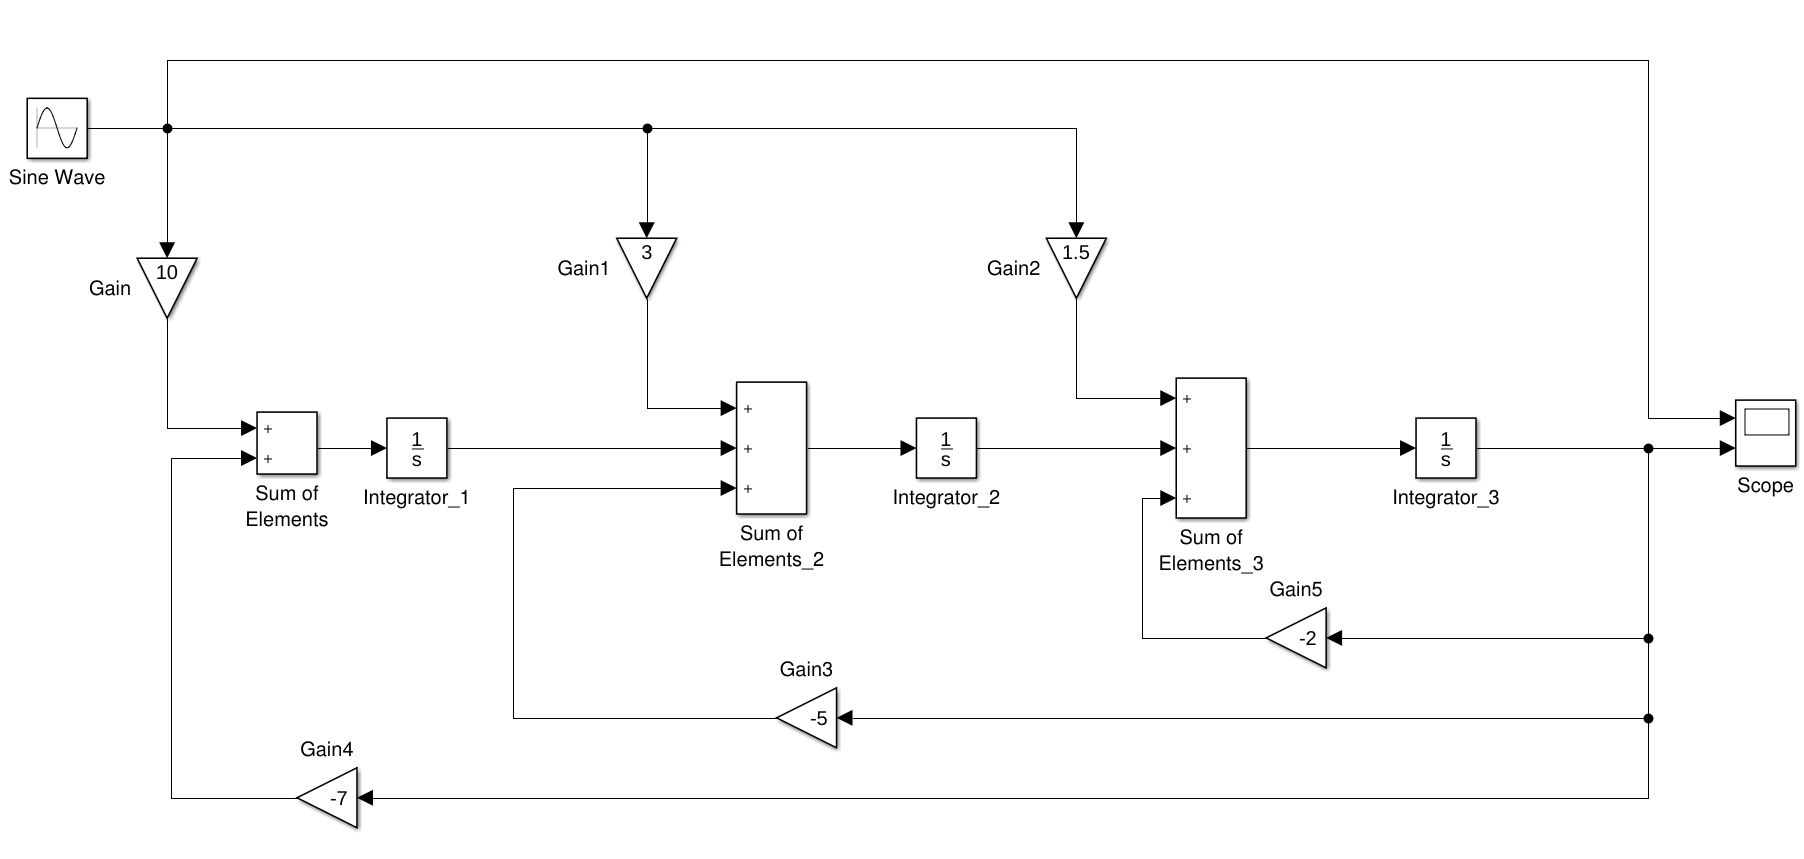
\includegraphics[scale=0.25]{SineWave}
		\caption{схема моделирования $u(t) = 2sin(t)$} 
		\label{pic:pic_1} % название для ссылок внутри кода
	\end{center}
\end{figure}

\begin{figure}[H]
	\begin{center}
		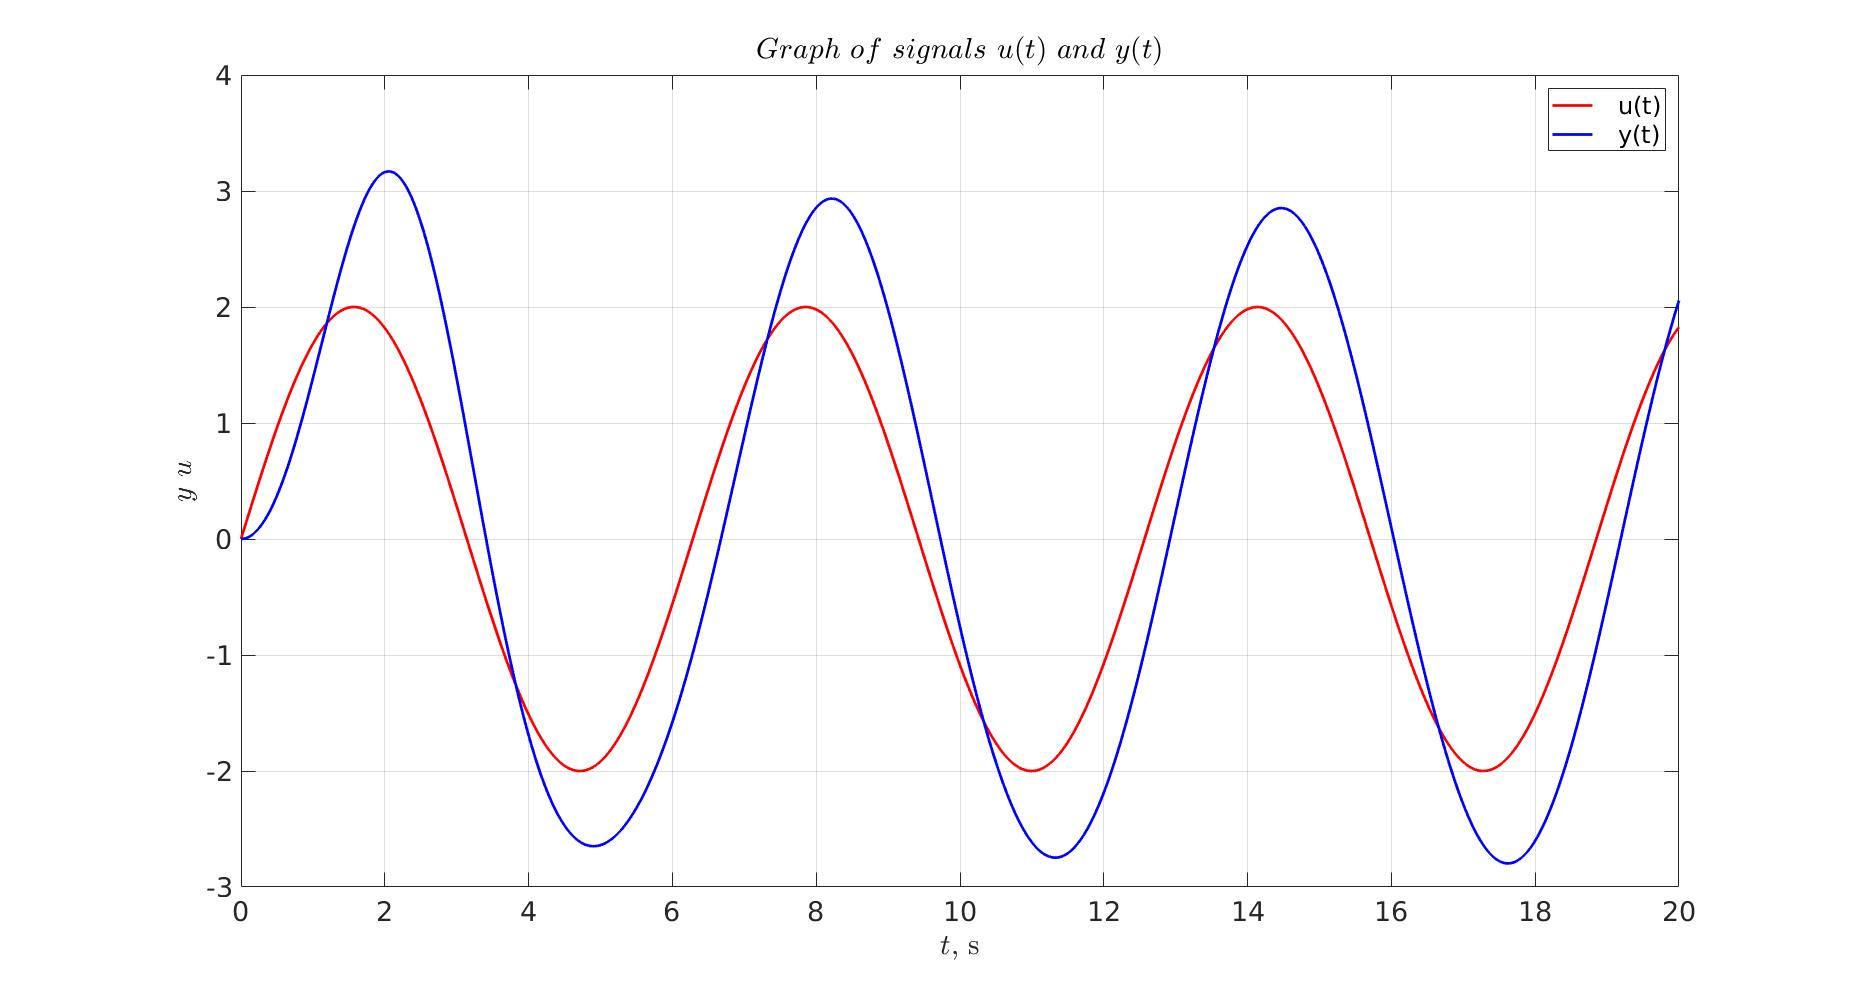
\includegraphics[scale=0.25]{SineWaveZeroCondition}
		\caption{графики сигналов $u(t)$ и $y(t)$} 
		\label{pic:pic_2} % название для ссылок внутри кода
	\end{center}
\end{figure}

\begin{figure}[H]
	\begin{center}
		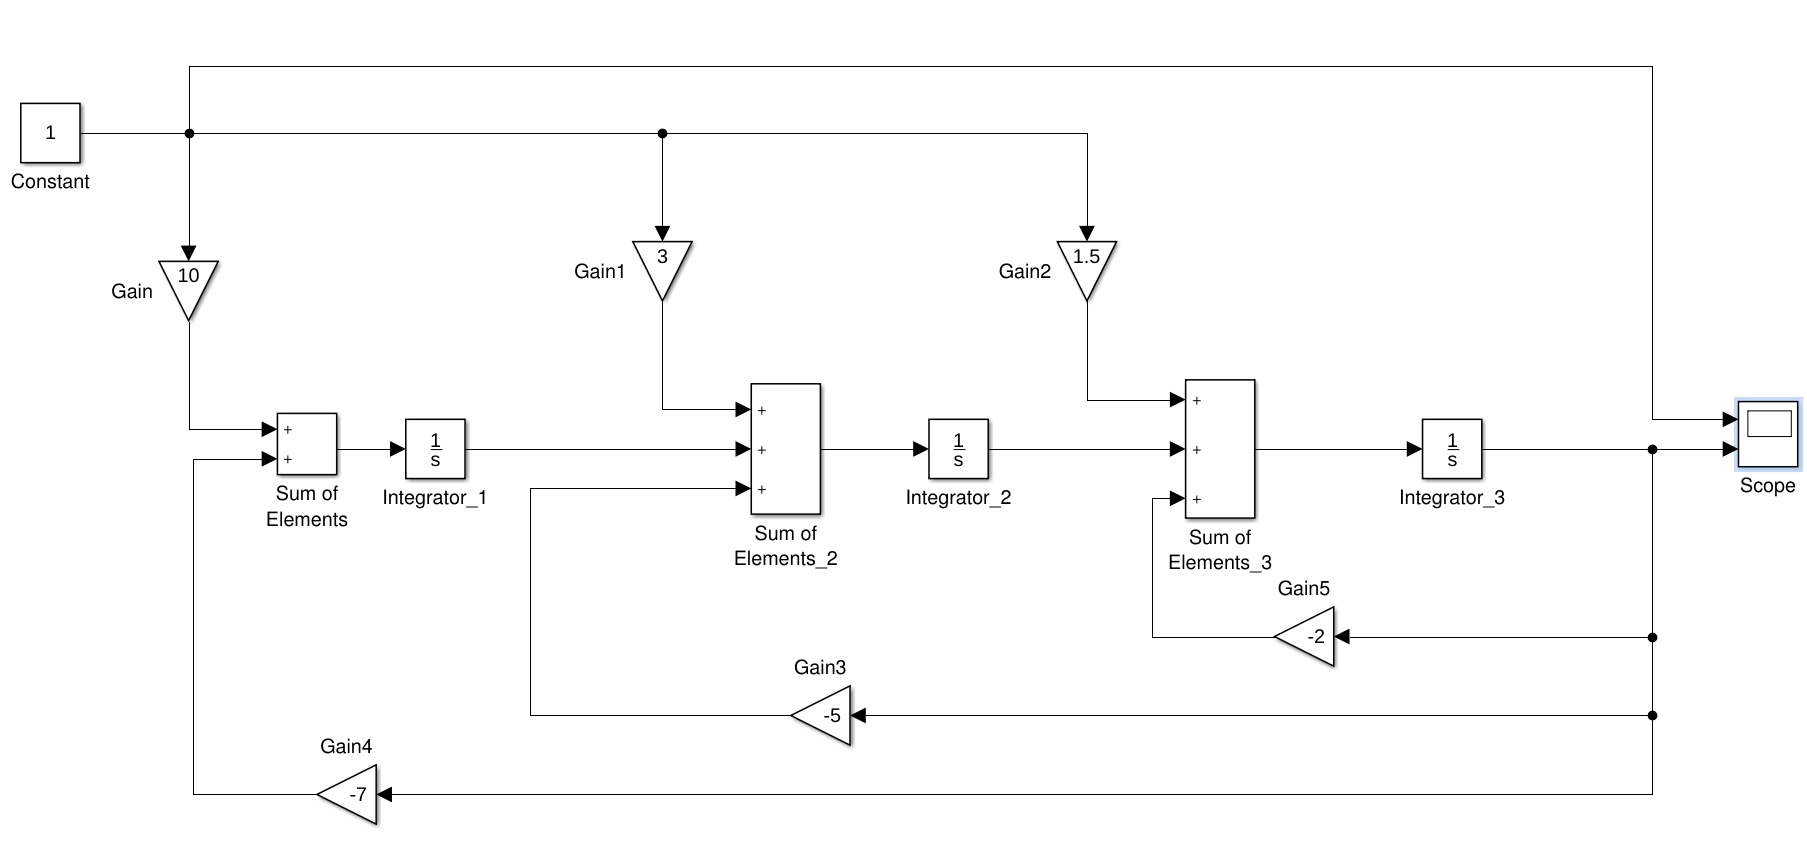
\includegraphics[scale=0.25]{Const}
		\caption{схема моделирования $u(t) = 1$} 
		\label{pic:pic_3} % название для ссылок внутри кода
	\end{center}
\end{figure}

\begin{figure}[H]
	\begin{center}
		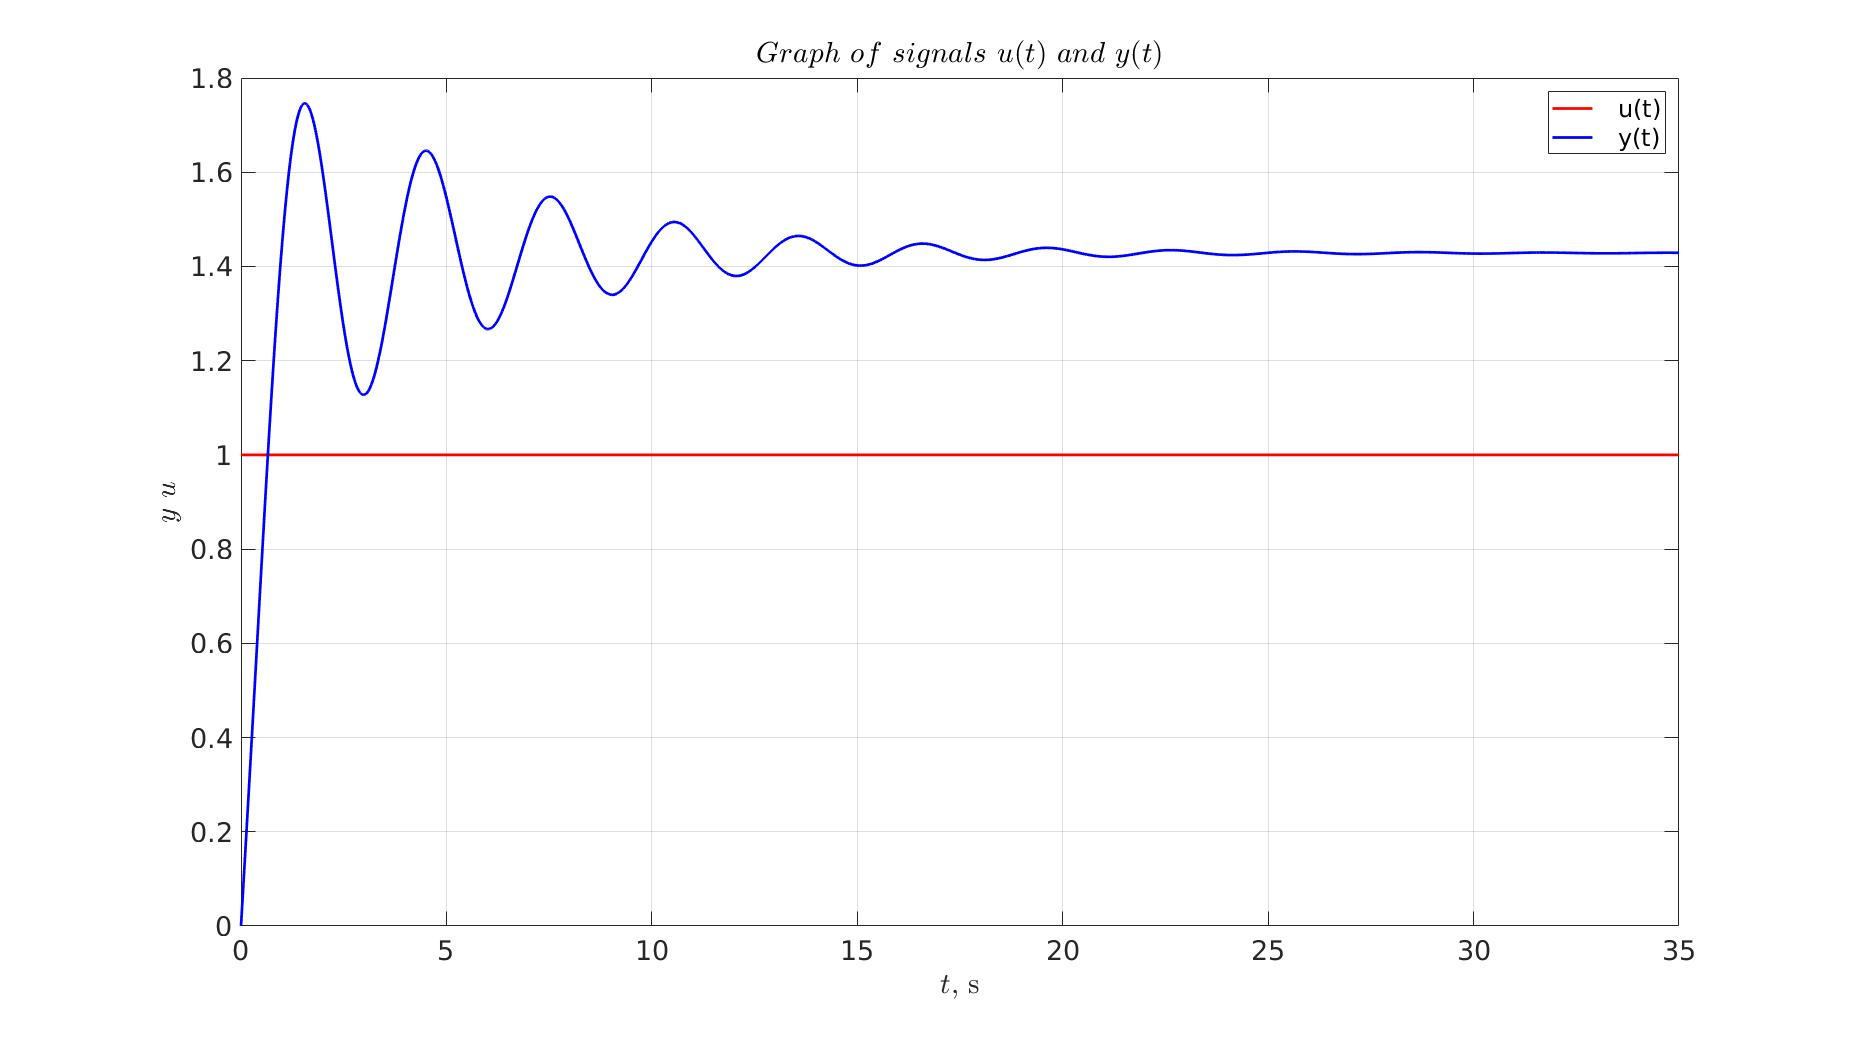
\includegraphics[scale=0.25]{ConstZeroCondition}
		\caption{графики сигналов $u(t)$ и $y(t)$} 
		\label{pic:pic_4} % название для ссылок внутри кода
	\end{center}
\end{figure}

\subsubsection{Моделирование свободного движения системы, т.е. с нулевым входным воздействием и ненулевыми начальными условиям:}

\begin{figure}[H]
	\begin{center}
		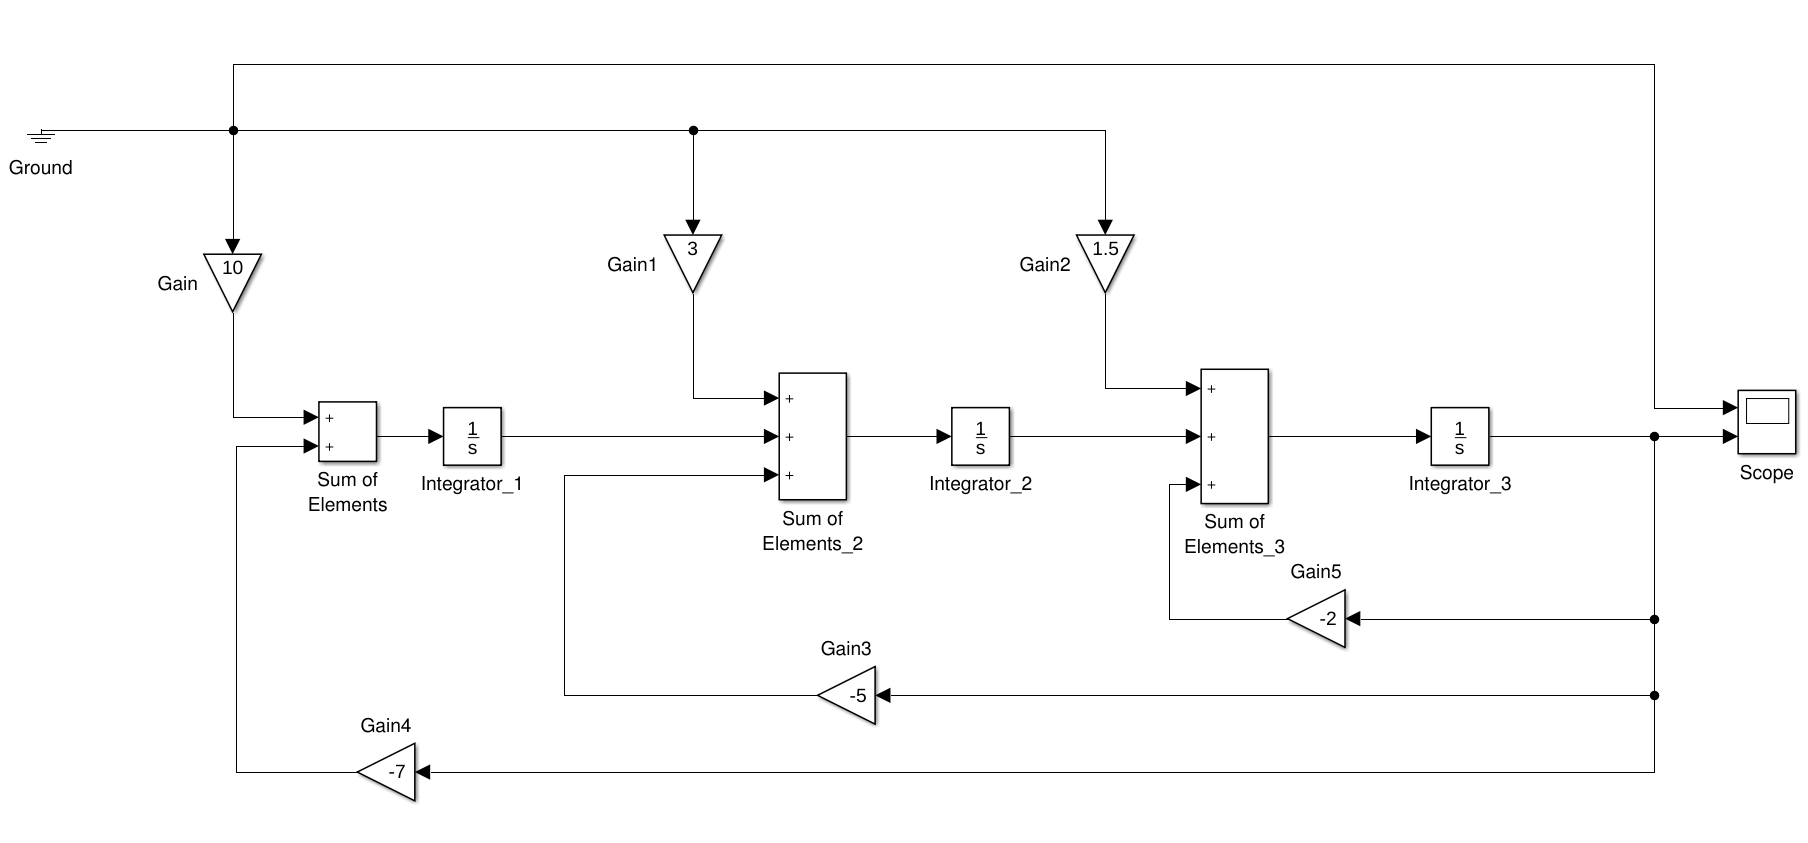
\includegraphics[scale=0.25]{ZeroImpactNoZeroConditionSimulink}
		\caption{схема моделирования с нулевым входным воздействием} 
		\label{pic:pic_5} % название для ссылок внутри кода
	\end{center}
\end{figure}

\begin{figure}[H]
	\begin{center}
		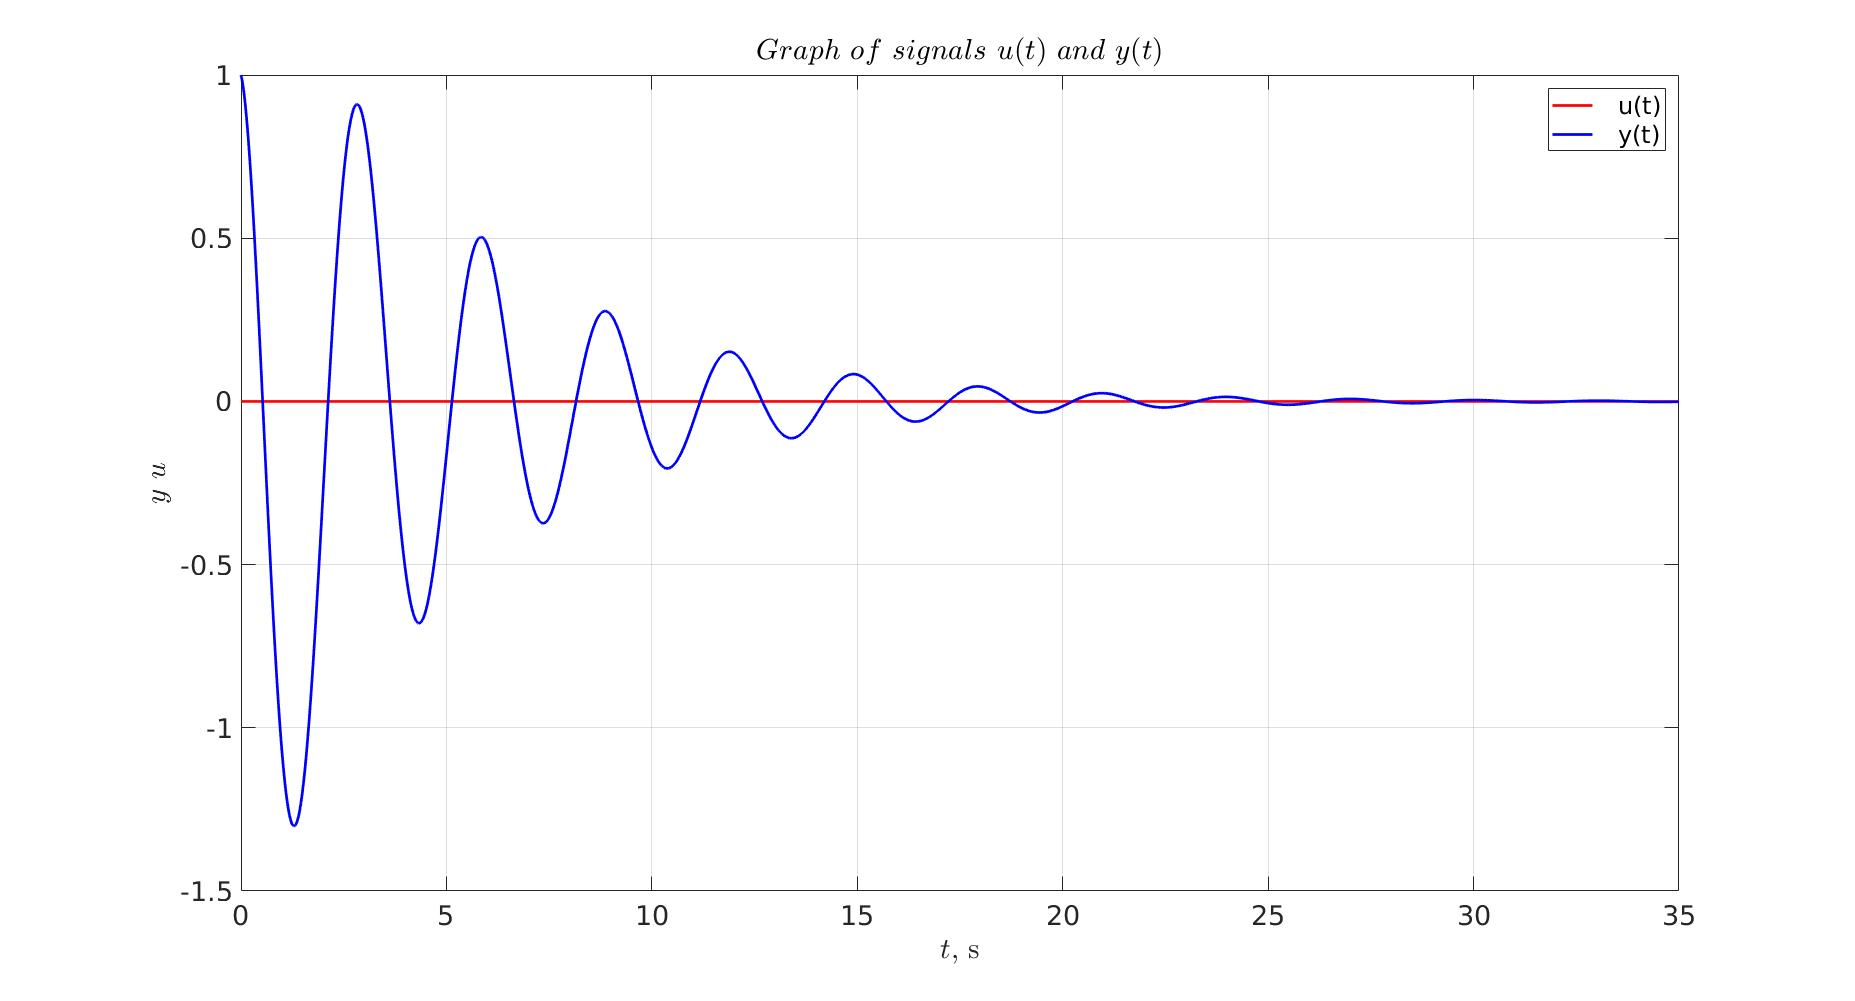
\includegraphics[scale=0.25]{ZeroImpactNoZeroCondition}
		\caption{график сигнала $y(t)$} 
		\label{pic:pic_6} % название для ссылок внутри кода
	\end{center}
\end{figure}

\newpage

\subsection{Модель вход-состояние-выход}
\subsubsection{Математическая модель:}

\begin{equation}
    \begin{matrix}
    \left\{
    \begin{matrix}
    \dot{x_1} = x_2 + 0.5u\\
    \dot{x_2} = -5x_1 - 0.5x_2 + u\\
    y = 5x_1 + 0.5x_2
    \end{matrix} \right.
    \end{matrix}
\end{equation}

\subsubsection{Моделирование системы при двух видах входного воздействия u = 2sin(t)  и u = 1(t) и нулевых начальных условиях:}

\begin{figure}[H]
	\begin{center}
		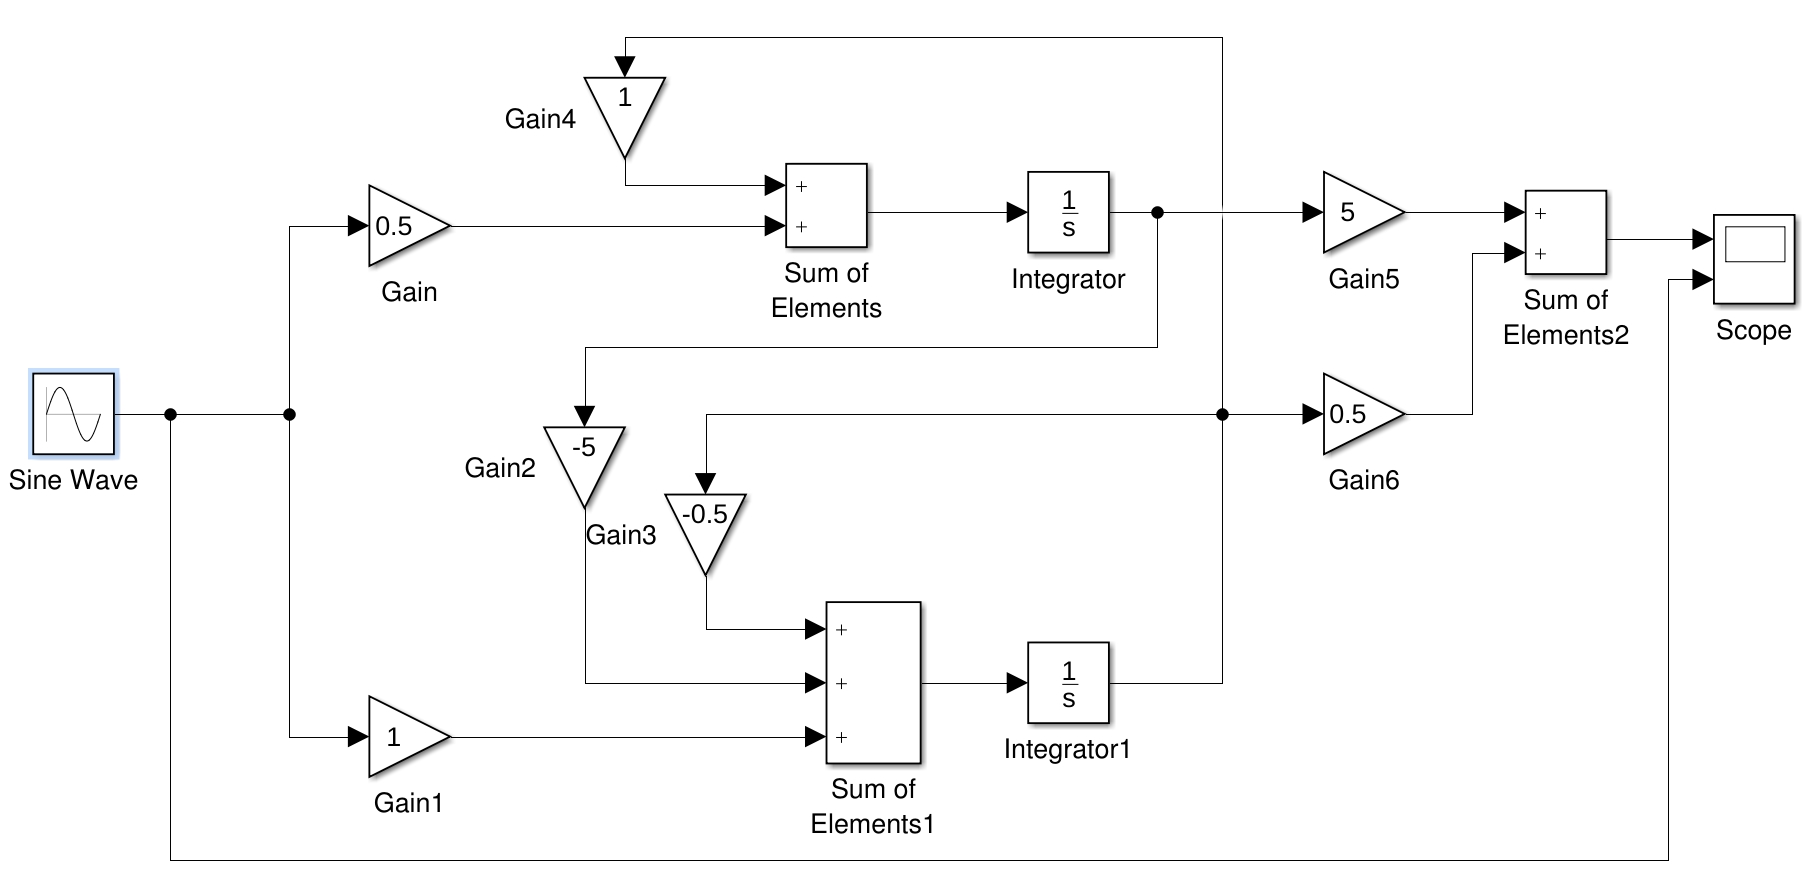
\includegraphics[scale=0.25]{SineWaveZeroConditionSim_2}
		\caption{схема моделирования $u(t) = 2sin(t)$} 
		\label{pic:pic_7} % название для ссылок внутри кода
	\end{center}
\end{figure}

\begin{figure}[H]
	\begin{center}
		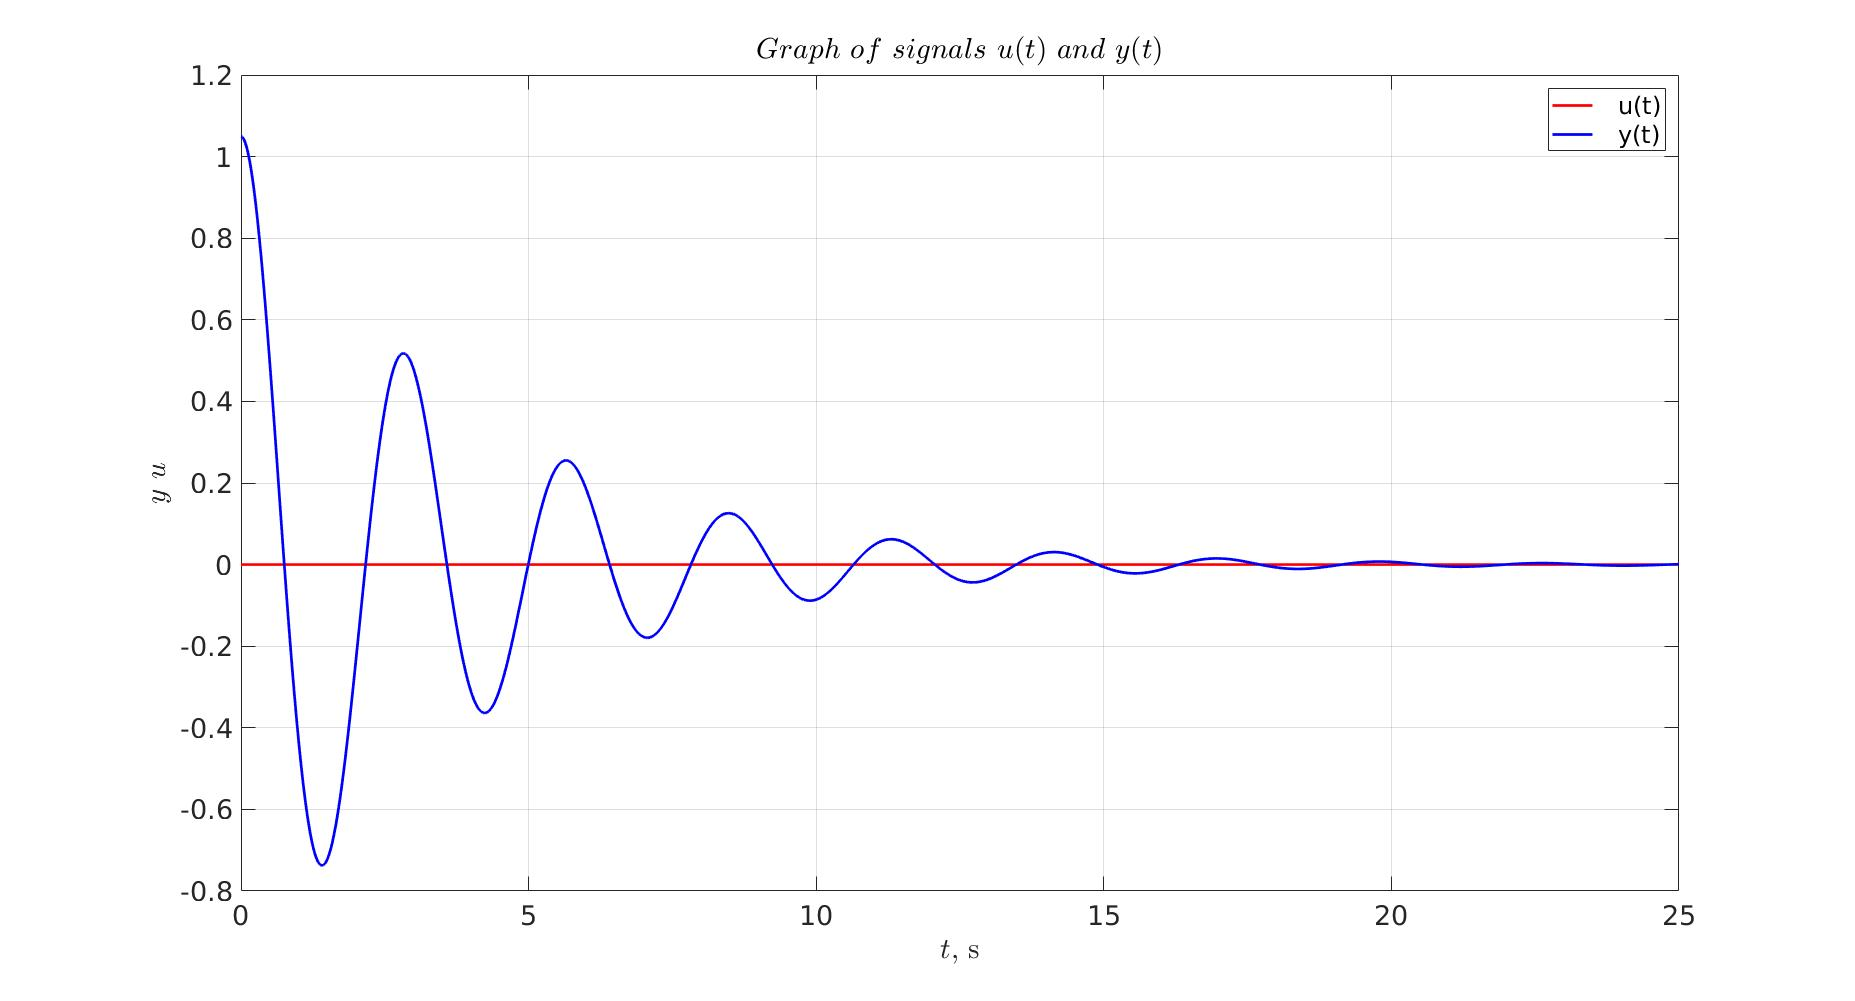
\includegraphics[scale=0.25]{SineWaveZeroCOndition_2}
		\caption{графики сигналов $u(t)$ и $y(t)$} 
		\label{pic:pic_8} % название для ссылок внутри кода
	\end{center}
\end{figure}

\begin{figure}[H]
	\begin{center}
		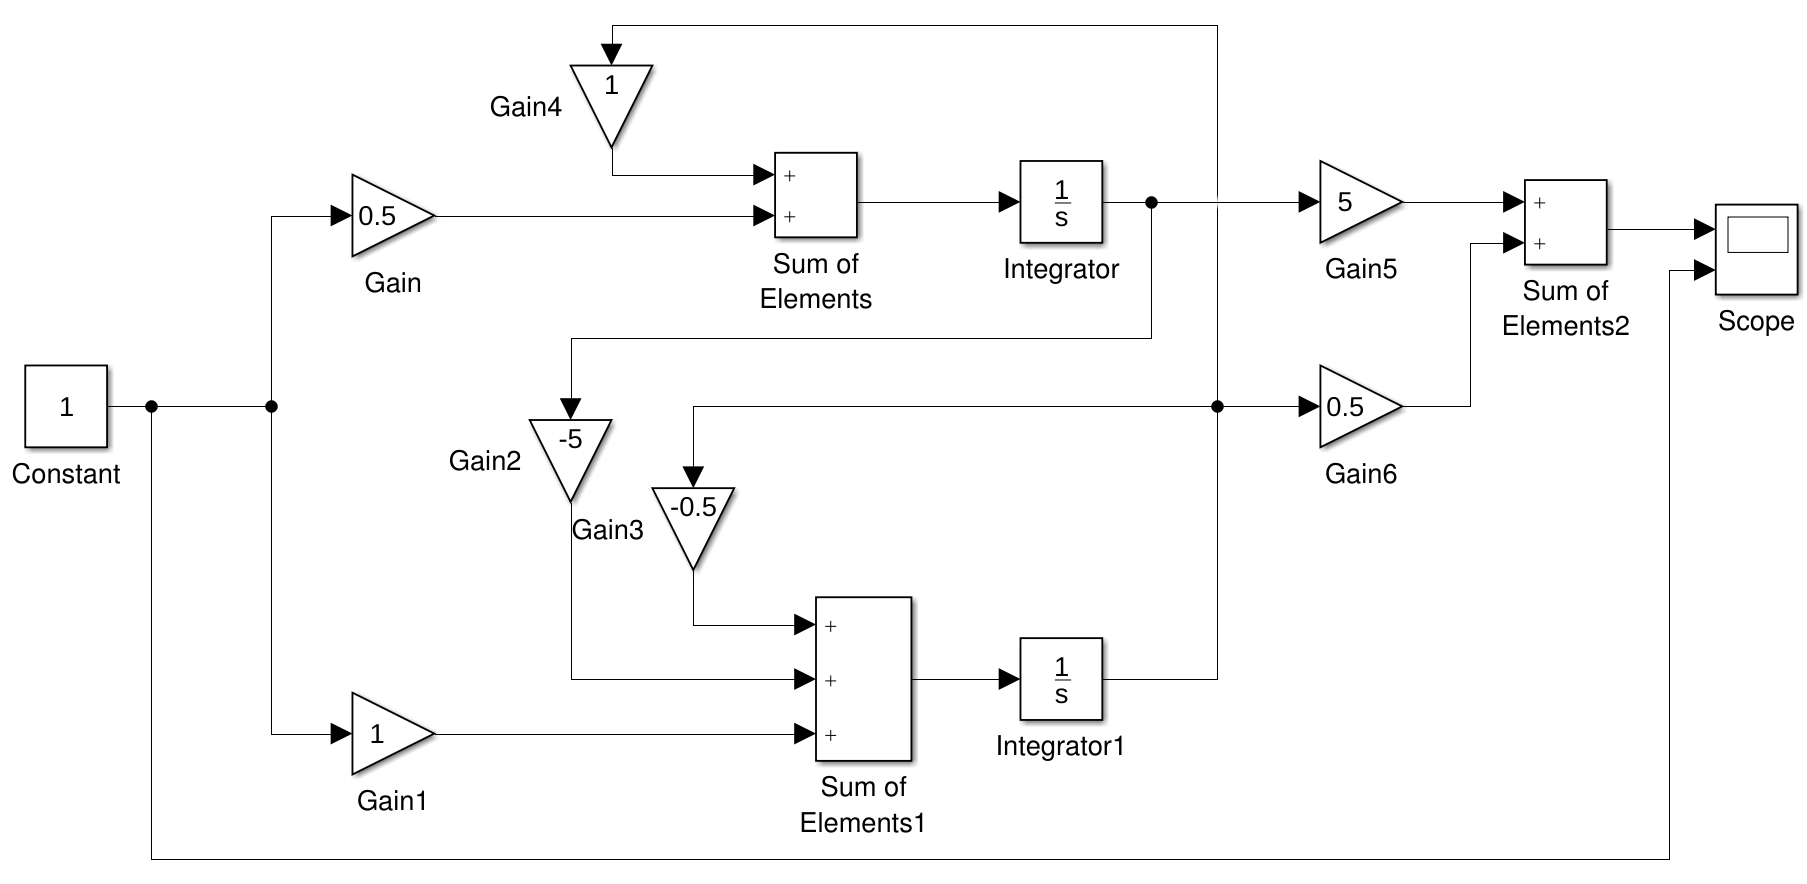
\includegraphics[scale=0.25]{ConstZeroConditionSim_2}
		\caption{схема моделирования $u(t) = 1$} 
		\label{pic:pic_9} % название для ссылок внутри кода
	\end{center}
\end{figure}

\begin{figure}[H]
	\begin{center}
		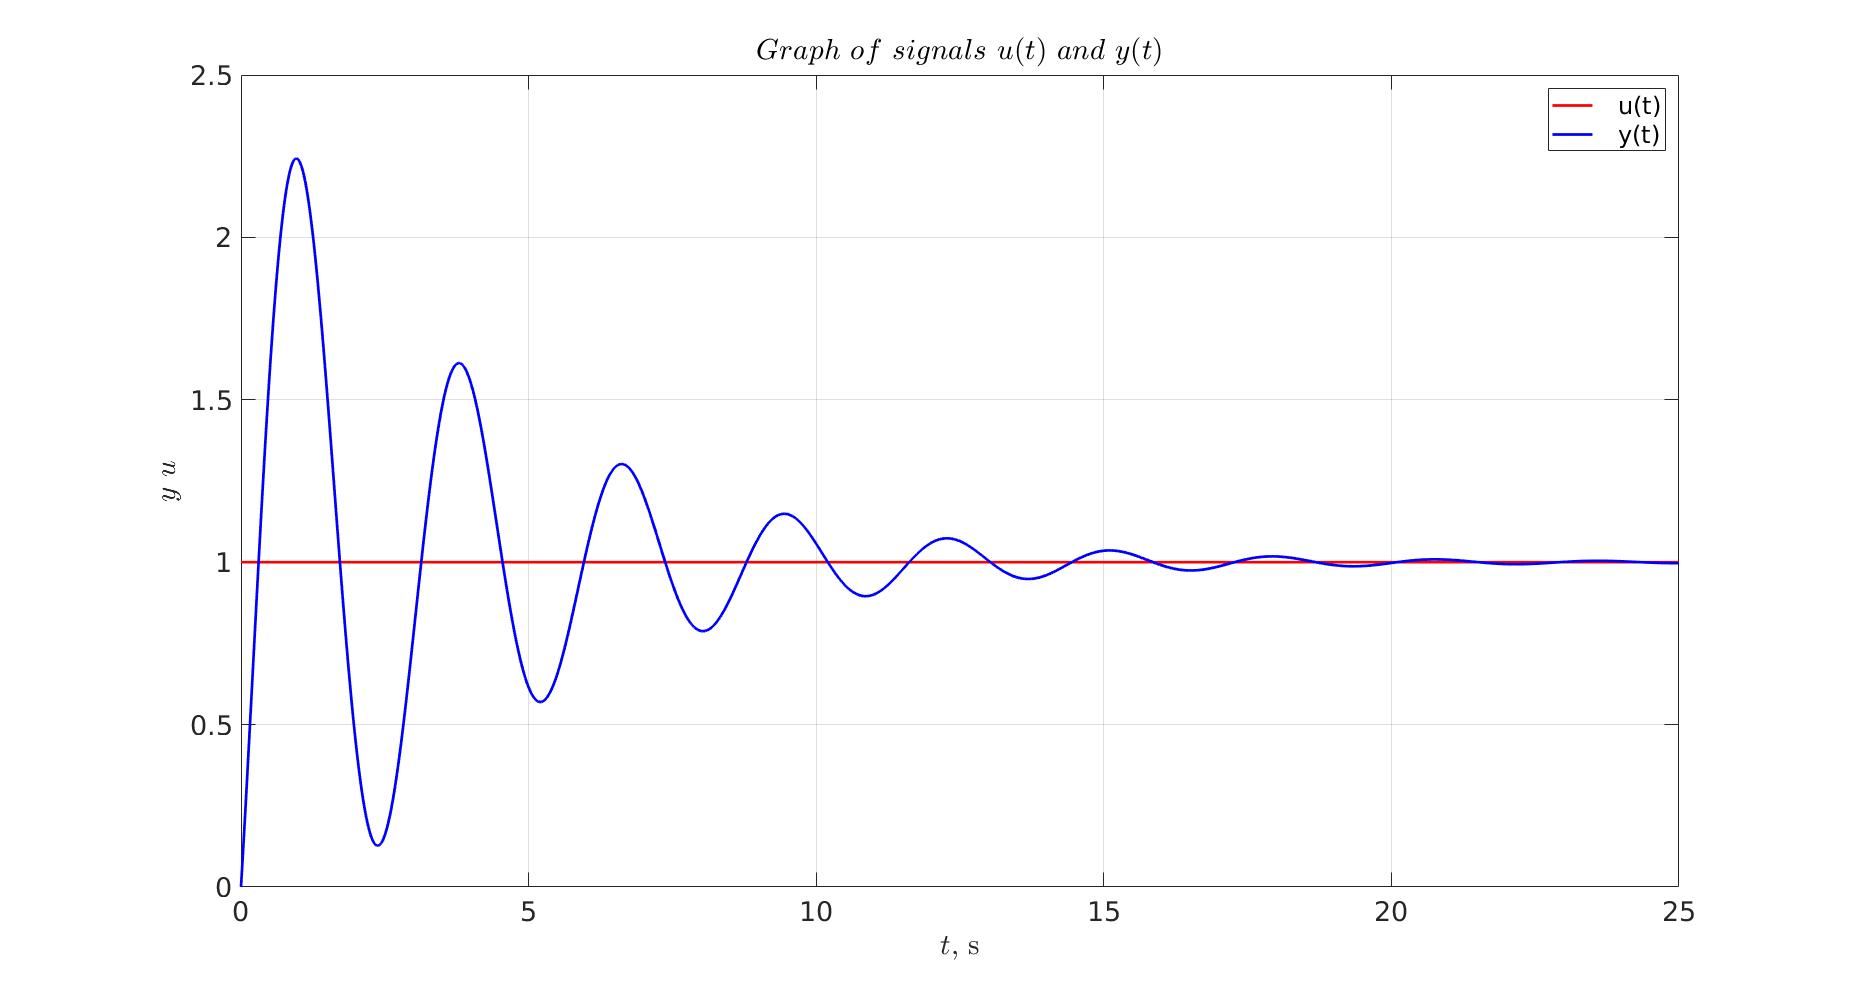
\includegraphics[scale=0.25]{ConstZeroCondition_2}
		\caption{графики сигналов $u(t)$ и $y(t)$} 
		\label{pic:pic_10} % название для ссылок внутри кода
	\end{center}
\end{figure}

\subsubsection{Моделирование свободного движения системы, т.е. с нулевым входным воздействием и ненулевыми начальными условиям:}

\begin{figure}[H]
	\begin{center}
		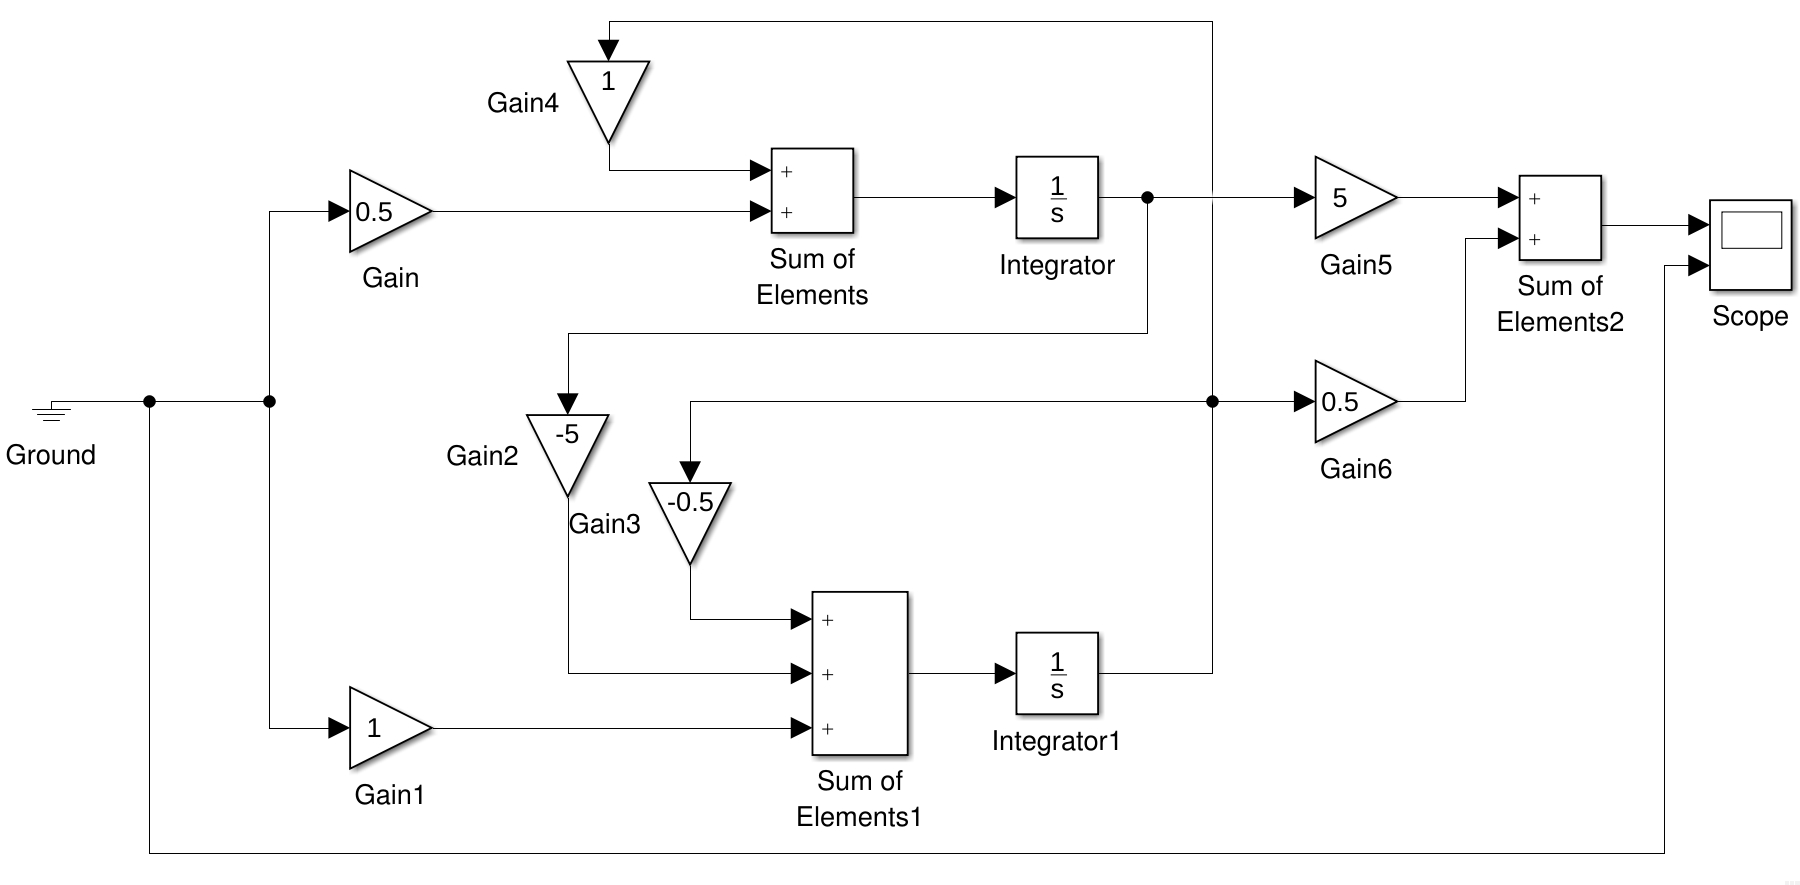
\includegraphics[scale=0.25]{ZeroImpactNoZeroConditionSim_2}
		\caption{схема моделирования с нулевым входным воздействием} 
		\label{pic:pic_11} % название для ссылок внутри кода
	\end{center}
\end{figure}

\begin{figure}[H]
	\begin{center}
		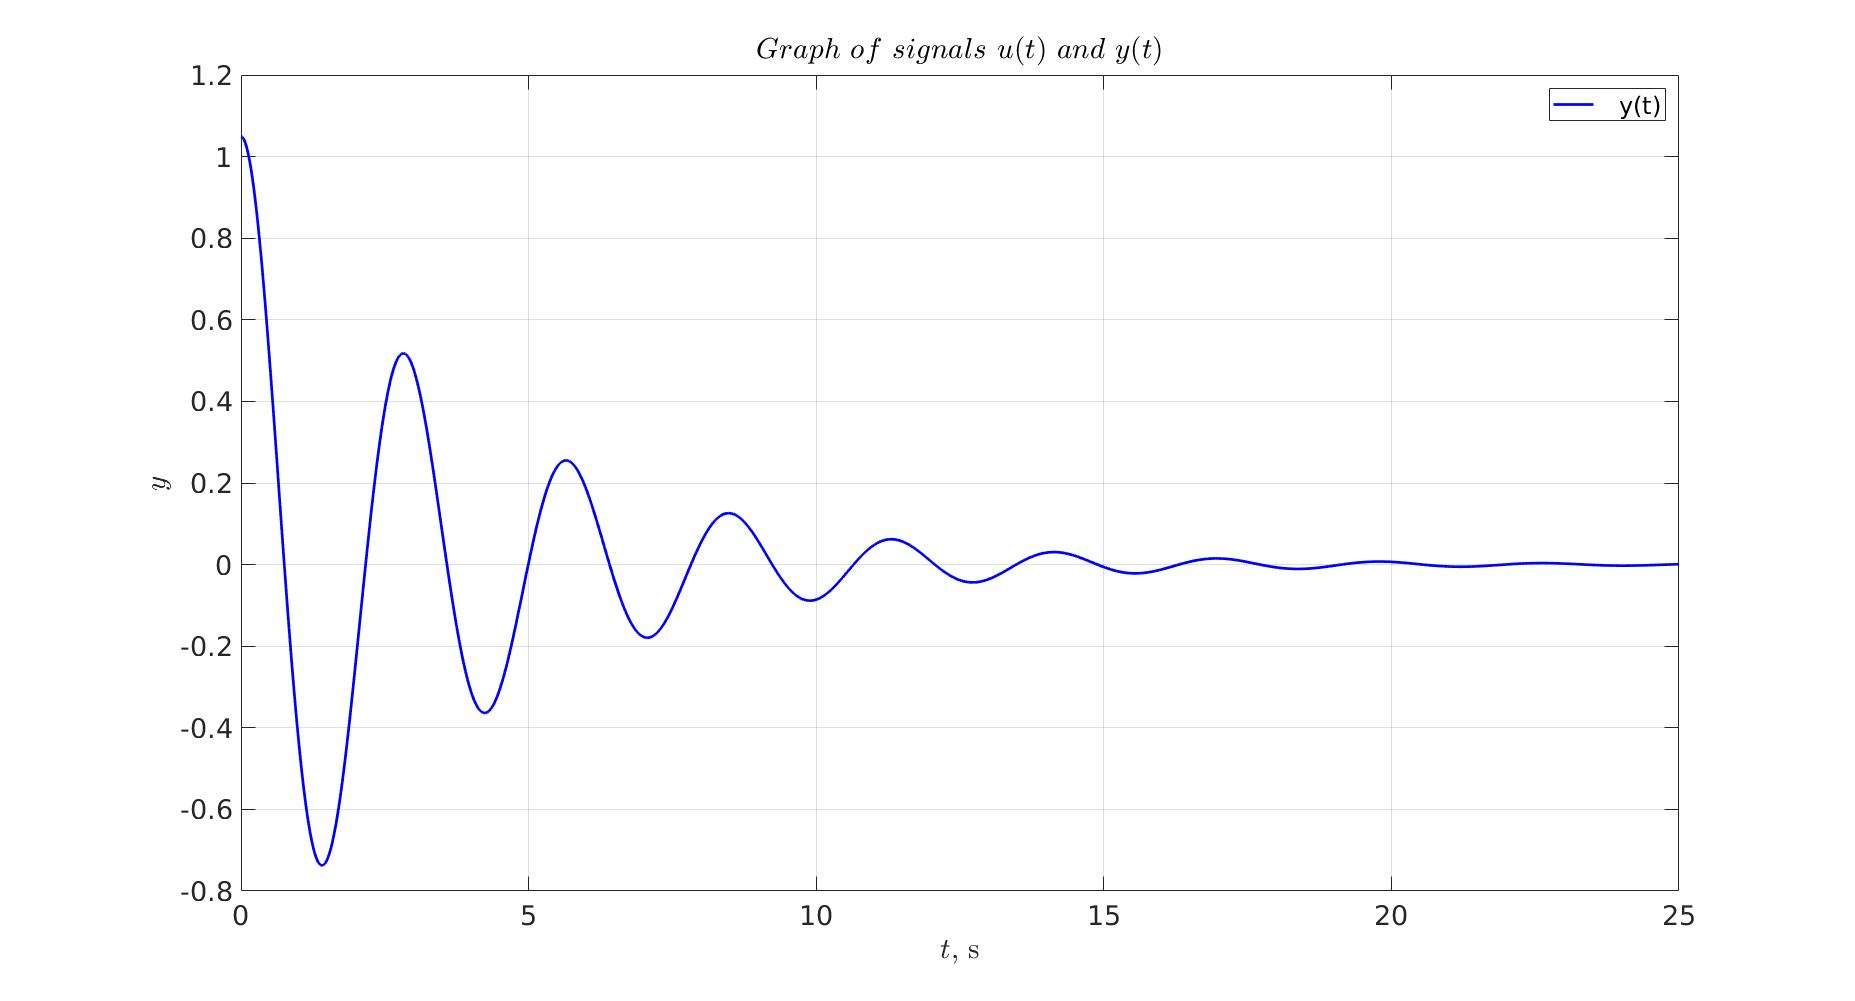
\includegraphics[scale=0.25]{ZeroImpactNoZeroCondition_2}
		\caption{график сигнала $y(t)$}
		\label{pic:pic_12} % название для ссылок внутри кода
	\end{center}
\end{figure}


\section{Создание графиков}

\lstinputlisting[
	label=code:plot,
	caption={plot.m},% для печати символ '_' требует выходной символ '\'
]{plot.m}
\parindent=1cm % командна \lstinputlisting сбивает параментры отступа

\newpage

\section{Вывод}
В данной лабораторной работе было знакомство с базовыми функциями пакета прикладных программ для решения задач технических вычислений - Matlab. Также были приобретены навыки в работе с графической средой имитационного моделирования - Simulink. Было знакомство с основными приемами моделирования линейных динамических систем. Было проведено моделирование системы вход-выход и вход-состояние-выход при различных видах входного воздействия - u = 1 и u = 2sin(t) и нулевыми начальными условиями, а также свободного движения системы. Также были построены графики входных и выходных сигналов. При исследовании модели вход-состояния-выход все системы пришли к состояния равновесия. Рисунки \ref{pic:pic_8}, \ref{pic:pic_10}, \ref{pic:pic_12}. А при исследовании модели вход-выход с входным сигналом u = 2sin(t) получили незатухающие колебания, что говорит о нестабильности системы \ref{pic:pic_2}. При двух других случаях были получены модели, которые пришли к состоянию равновесия \ref{pic:pic_4} и \ref{pic:pic_6}.
\end{document}
